\chapter{查询优化}
在实际的操作中,不同的查询需要采取不同的实现方法。有时候查询语句往往一个小的改动都会造成完全不一样的时间消耗,这一点在大型数据上的表现尤其的明显。所以,在实际的执行过程中要特别注重查询的效率问题,结合数据库理论和具体的环境进行不同的优化工作。优化的方法有很多种,根据我的查找和思考,以及\cite{youhua},\cite{youhuayanjiu},\cite{hiveperformemce},\cite{youhuaqi}的介绍,这里仅仅介绍我个人认为比较重要的几个方面。

\section{使用索引}
我们知道,索引是数据库中十分重要的一个概念,如果使用的合理适当,能够极大幅度的提高效率。从某种意义上来说,索引可以理解为一种特殊的目录。索引中保存着表中存储的索引列,并且记录了索引列在数据库表中的物理存储位置,实现了表中数据的逻辑索引。在没有索引时,查询需要进行全表的扫描,将每一条的记录取出并和查询条件一一对比,这无疑会消耗大量的时间并且造成许多磁盘IO。有了索引之后,就可以直接在索引中找到符合条件的索引值,将相应的指针返回就能够找到需要的记录。因此,有了索引可以避免全表扫描,也就可以大大减少时间。这和通过目录查找相应的内容的道理是一样的,要比一页一页的翻肯定来得快。


需要注意的是,索引也是一个单独的物理结构,建立索引需要花费空间和时间的代价,它也是要占用物理空间的。更加重要的是,一旦表中的记录发生了变化如增加删除和修改等等,索引本身也要相应的调整,因此要适当考虑创建和维护索引的代价,想好究竟哪些字段需要建立索引,不能一味建立索引。


事实上,索引的建立是有一定的原则的。如对于查询中很少涉及到的列或者重复值比较多的列不需要建立索引;对于按范围查询的列最好建立索引;表中若有主键或者外键一定要建立索引;而对于一些特殊的数据类型,如文本字段TXT,图像类型字段IMAGE等等,由于长度不定,很难建立索引。


一般数据库中的索引分为唯一索引、主键索引和聚集索引。唯一索引就是不允许任何两行有相同索引值的索引;主键索引是为主键所准备,它唯一表示了这一行;聚集索引是使得表的索引顺序和物理顺序一样,一个表只能包含一个聚集索引。


根据索引的特点一般来说,下面的几种情况下建立索引最为有效:
\begin{compactitem}
\item
在经常进行连接的字段上建立索引。
\item
在频繁进行groupby 和orderby,即排序或者分组操作的列上建立索引。
\item
在条件表达式中经常用到的不同值较多的列上建立索引。
\item
如果待排序的列有多个,可以在这些列上建立复合索引。
\end{compactitem}

接下来我们通过一个例子来验证索引的作用:

\begin{lstlisting}[language=SQL]
// 查询语句 
select calldate,time from duanxin where calldate>100600 and time>110000 group by calldate;

// 建立索引 
create index date_time on duanxin(calldate(6),time(6));

// 使用索引 
select calldate,time from duanxin force index(date_time) where calldate>100600 and time>110000 group by calldate;
\end{lstlisting}

下面是建立索引前后的对比:
\begin{figure}[h]
\begin{minipage}[t]{0.4\linewidth}
\centering
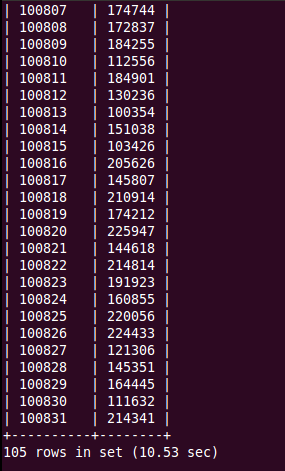
\includegraphics[width=0.7\textwidth,height=7cm]{photo/index1.png}
\caption{建立索引前}
\end{minipage}
\hfill
\begin{minipage}[t]{0.4\linewidth}
\centering
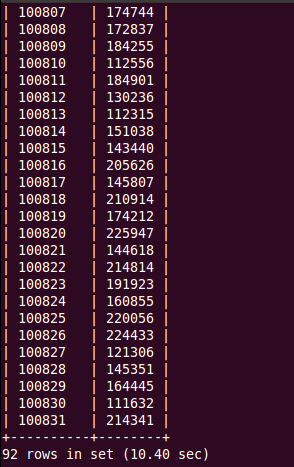
\includegraphics[width=0.7\textwidth,height=7cm]{photo/index2.png}
\caption{建立索引后}
\end{minipage}
\end{figure}

\section{参数优化}
在实际应用中,设定参数可以调优查询代码的执行效率。这里仅仅讨论hive的参数优化问题。

\subsection{如何设定参数}
首先说明的是,对于一般的参数,大概有三种设定方式:
\begin{compactitem}
\item 配置文件
\item 命令行参数
\item 参数声明
\end{compactitem}
其中配置文件就是conf文件夹下的文件,可以是默认的,也可以是用户自己定义的配置文件。配置文件的设定对本机启动的所有Hive进程都有效。而命令行参数就是在启动hive时,在命令行添加 -hiveconf param=value来设定。参数声明就是在HQL中使用SET关键字设定,如set mapred.reduce.tasks=100.后两种设定的作用域是Session级的。

\subsection{列裁剪(Column Pruning)}
在读数据的时候,只读取查询中需要的列,而忽略其他列。例如表T 包含 5 个列 (a,b,c,d,e),当实现查询

\begin{lstlisting}[language=SQL]
SELECT a,b FROM T WHERE e < 10;
\end{lstlisting}

这样列 c,d 将会被忽略,只会读取a, b, e 列。这个选项默认为真:hive.optimize.cp = true

\subsection{分区裁剪(Partition Pruning)}
在查询时减少不必要的分区。例如:

\begin{lstlisting}[language=SQL]
SELECT * FROM (SELECT c1, COUNT(1)
  FROM T GROUP BY c1) subq
  WHERE subq.prtn = 100;

SELECT * FROM T1 JOIN
  (SELECT * FROM T2) subq ON (T1.c1=subq.c2)
  WHERE subq.prtn = 100;
\end{lstlisting}

会在子查询中就考虑 subq.prtn = 100 条件,从而减少读入的分区数目。
此选项默认为真:hive.optimize.pruner=true。

\subsection{Join和MapJoin}
首先应该将条目少的表/子查询放在 Join 操作符的左边。因为join操作符左边的表的内容会被加载进内存。另外,在多个表进行join时,如果join的key值是相同的,那么将会合并成一个MapReduce任务,如果不同,则任务数目和join操作的数目相同。


join的方法有reduce端的join和map端的join之分,其中reduce端的join的工作就是把两个表都生成key-value对,在reduce端进行笛卡尔积;mapjoin的原理就是把小表全部读入内存中,在map阶段直接拿另外一个表的数据和内存中表数据做匹配。换句话说,只将大表生成key-value对,由于小表非常的小,足以在内存中放下并且可以进行全表的扫描,因此在map端就可以将小表中的值全部取出并匹配,避免了笛卡尔乘积。\cite{mapjoin}.


下面是一个使用mapjoin的例子:

\begin{lstlisting}[language=SQL]
SELECT /*+ MAPJOIN(x) */ x.key, x.value, y.valueFROM src1 x LEFT OUTER JOIN src y ON (x.key = y.key);
\end{lstlisting}

再次强调mapjoin仅仅适用于一个小表和一个大表join的场景。因此这里的表x一定是小表。如果太大会出现内存不足的错误。

\subsection{groupby}
hive.map.aggr = true 是否在 Map 端进行聚合,默认为 True 
hive.groupby.mapaggr.checkinterval = 100000 在 Map 端进行聚合操作的条目数目 
hive.groupby.skewindata = false 有数据倾斜的时候进行负载均衡 

\subsection{合并小文件}
文件数目过多,会给 HDFS 带来压力,并且会影响处理效率,可以通过合并 Map 和 Reduce 的结果文件来消除这样的影响:
\begin{compactitem}
\item hive.merge.mapfiles = true 是否和并 Map 输出文件,默认为 True 
\item hive.merge.mapredfiles = false 是否合并 Reduce 输出文件,默认为 False 
\item hive.merge.size.per.task = 256*1000*1000 合并文件的大小 
\end{compactitem}

\section{解决数据倾斜}
数据倾斜的原因是在map端处理数据量的差异太大,进而导致数据无法均匀的分配到各个reduce中。数据倾斜有很多种情形,比如说join时的key值分布不均匀,或者join时存在很多的空值。因为Hive中,主键为null值的项会被当做相同的Key而分配进同一个计算Map。另外还有groupby或者count distinct时某些值太多导致处理这个值的reduce非常的耗时。解决的方法有很多种,比如对于join时存在很多空值的情况,在sql语句中设置值不为空的不参与关联,或者把空值的key变成一个字符串加上随机数,把倾斜的数据分到不同的reduce上,由于null值关联不上,处理后并不影响最终结果。对于count distinct情况,可以利用group by替代它达到效果。比如说这样改:
\begin{lstlisting}[language=SQL]
//count(distinct)sql 语句
select address,count(distinct number)
from duanxin
group by address;

//替换的group by 语句
select address,count(1)
from (
select address
from duanxin
group by address,number
) t
group by address;
\end{lstlisting}

下面两个图是两个方法得出的结果。
\begin{figure}[h]
\begin{minipage}[t]{0.45\linewidth}
\centering
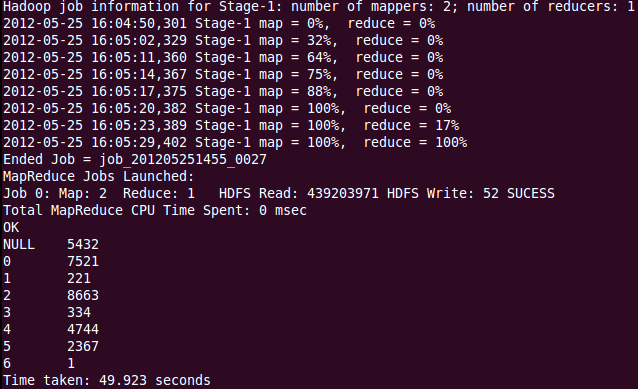
\includegraphics[width=0.8\textwidth,height=5cm]{photo/qxbefore.png}
\caption{使用cout(distinct)}
\end{minipage}
\hfill
\begin{minipage}[t]{0.45\linewidth}
\centering
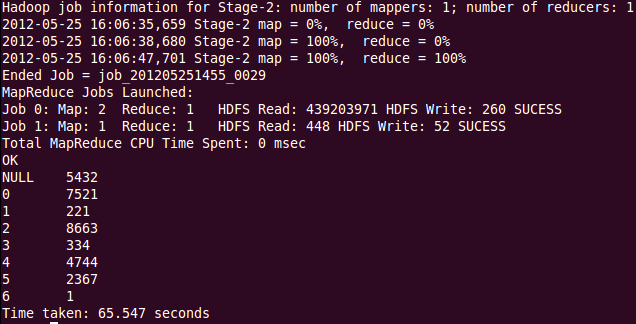
\includegraphics[width=0.8\textwidth,height=5cm]{photo/qxafter.png}
\caption{使用group by代替之}
\end{minipage}
\end{figure}
由于这里第一数据量不是特别大,第二数据倾斜不是很严重,第三替换后的增加了子查询的操作所以才会出现前者时间比后者多的情况。

\section{对join查询算法的研究}
参考文献\cite{join}比较详细的介绍了各种join的算法。标准的join算法可以通过MapReduce的一个Job实现。在map阶段通过提取需要join的key,生成一个标签tag,再加上value形成一个(key,value)对。这个标签标志了这条记录来源于哪一个表。接下来将他们进行排序与合并。在reduce阶段,对于每一个key,根据标签来把每一个value值划分为左右两个缓冲区,该记录来源于两个表中的哪个表就放到哪个缓冲区里。然后进行笛卡尔积就可以得到结果。伪代码可以表示为:
\begin{lstlisting}
Map(K:null,V:a record from a split of either R or L)
  join_key ← extract the join column from V
  tagged_record ← add a tag of either R or L to V
  emit(join_key,tagged_record)

Reduce(K′: a join key,LISTV′: r ecords from R and L with join key K′)
create buffers BR and BL for R and L, respectively
for each record t in LISTV′do
append t to one of the buffers according to its tag
for each pair of records (r, l) in BR×BL do
emit(null , newrecord(r,l))
\end{lstlisting}

这个算法的实现在hadoop自带的例子datajoin里面有。代码如下:
\begin{lstlisting}[language=Java]
//SampleDataJoinMapper.java
public class SampleDataJoinMapper extends DataJoinMapperBase {


  protected Text generateInputTag(String inputFile) {
    // tag the row with input file name (data source)
    return new Text(inputFile);
  }

  protected Text generateGroupKey(TaggedMapOutput aRecord) {
    // first column in the input tab separated files becomes the key (to perform the JOIN)
    String line = ((Text) aRecord.getData()).toString();
    String groupKey = "";
    String[] tokens = line.split("\\t", 2);
    groupKey = tokens[0];
    return new Text(groupKey);
  }

  protected TaggedMapOutput generateTaggedMapOutput(Object value) {
    TaggedMapOutput retv = new SampleTaggedMapOutput((Text) value);
    retv.setTag(new Text(this.inputTag));
    return retv;
  }
}

//SampleDataJoinReducer.java
public class SampleDataJoinReducer extends DataJoinReducerBase {
  protected TaggedMapOutput combine(Object[] tags, Object[] values) {
    // eliminate rows which didnot match in one of the two tables (for INNER JOIN)
    if (tags.length < 2)
       return null;  
    String joinedStr = ""; 
    for (int i=0; i<tags.length; i++) {
      if (i > 0)
         joinedStr += "\t";
      // strip first column as it is the key on which we joined
      String line = ((Text) (((TaggedMapOutput) values[i]).getData())).toString();
      String[] tokens = line.split("\\t", 2);
      joinedStr += tokens[1];
    }
    TaggedMapOutput retv = new SampleTaggedMapOutput(new Text(joinedStr));
    retv.setTag((Text) tags[0]); 
    return retv;
  }
}

//SampleDataOutput.java
public class SampleTaggedMapOutput extends TaggedMapOutput {

  private Text data;

  public SampleTaggedMapOutput() {
    this.data = new Text("");
  }

  public SampleTaggedMapOutput(Text data) {
    this.data = data;
  }

  public Writable getData() {
    return data;
  }

  public void write(DataOutput out) throws IOException {
    this.tag.write(out);
    this.data.write(out);
  }

  public void readFields(DataInput in) throws IOException {
    this.tag.readFields(in);
    this.data.readFields(in);
  }
}
\end{lstlisting}

这个算法的问题在于对两个表都需要进行缓冲,数据量很大时表不一定能完全放到内存缓冲区里。针对这个问题有许多种改进方法。第一个改进就是将标签放到value里,形成value\_tag的方式,这样便于对两个表分别进行排序。第二个改进就是无论在map阶段还是reduce阶段都对join\_key生成hash值,这样便于查找。最后的改进方法包括只将相对较小的表进行缓冲,然后再生成join的结果。
\begin{lstlisting}
Map(K: null , V: a record from a split of either R or L)
joinkey ← extract the join column from V
tagged record ← add a tag of either R or L to V
compositekey ← (joinkey, tag)
emit(compositekey, taggedrecord)
Partition(K: input key)
hashcode ← hashfunc(K.joinkey)
return hashcode mod # reducers

Reduce(K′: a composite key with the join key and the tag 
LISTV′: records for K′, first from R, then L)
create a buffer BR for R
for each R record r in LISTV′do
store r in BR
for each L record l in LISTV′do
for each record r in BR do
emit(null , newrecord(r, l))
\end{lstlisting}

还有一个改进可以是首先进行预处理操作,针对join\_key先进行分块,这样在以后的join操作之前都避免了相同操作,直接的进行join就行了。